% Emacs, this is -*-latex-*-

% Feeding the Team

\label{sec:feeding_the_team}

The splitter divides the stream into chunks of constant length $C$,
and sends exclusively each chunk to a different
\gls{origin}\footnote{In the route that a chunk traces from the
  splitter to all peers of the team, the origin peer is the first of
  this route i.e. the peer selected by the splitter for that chunk.}
peer, using a round-robin schema. Chunks are enumerated to distinguish
them. This information is transmitted as a part of a chunk header.

\begin{comment}
More details about the implementation
are available in Fig.~\ref{fig:chunk_generation}.

%$x$, conforming a message
%$c_x=[x,\text{chunk}]$, where
%$x=i \text{mod} \text{Splitter\_DBS.list\_of\_peers}.\text{length}()$.

\begin{figure*}
  %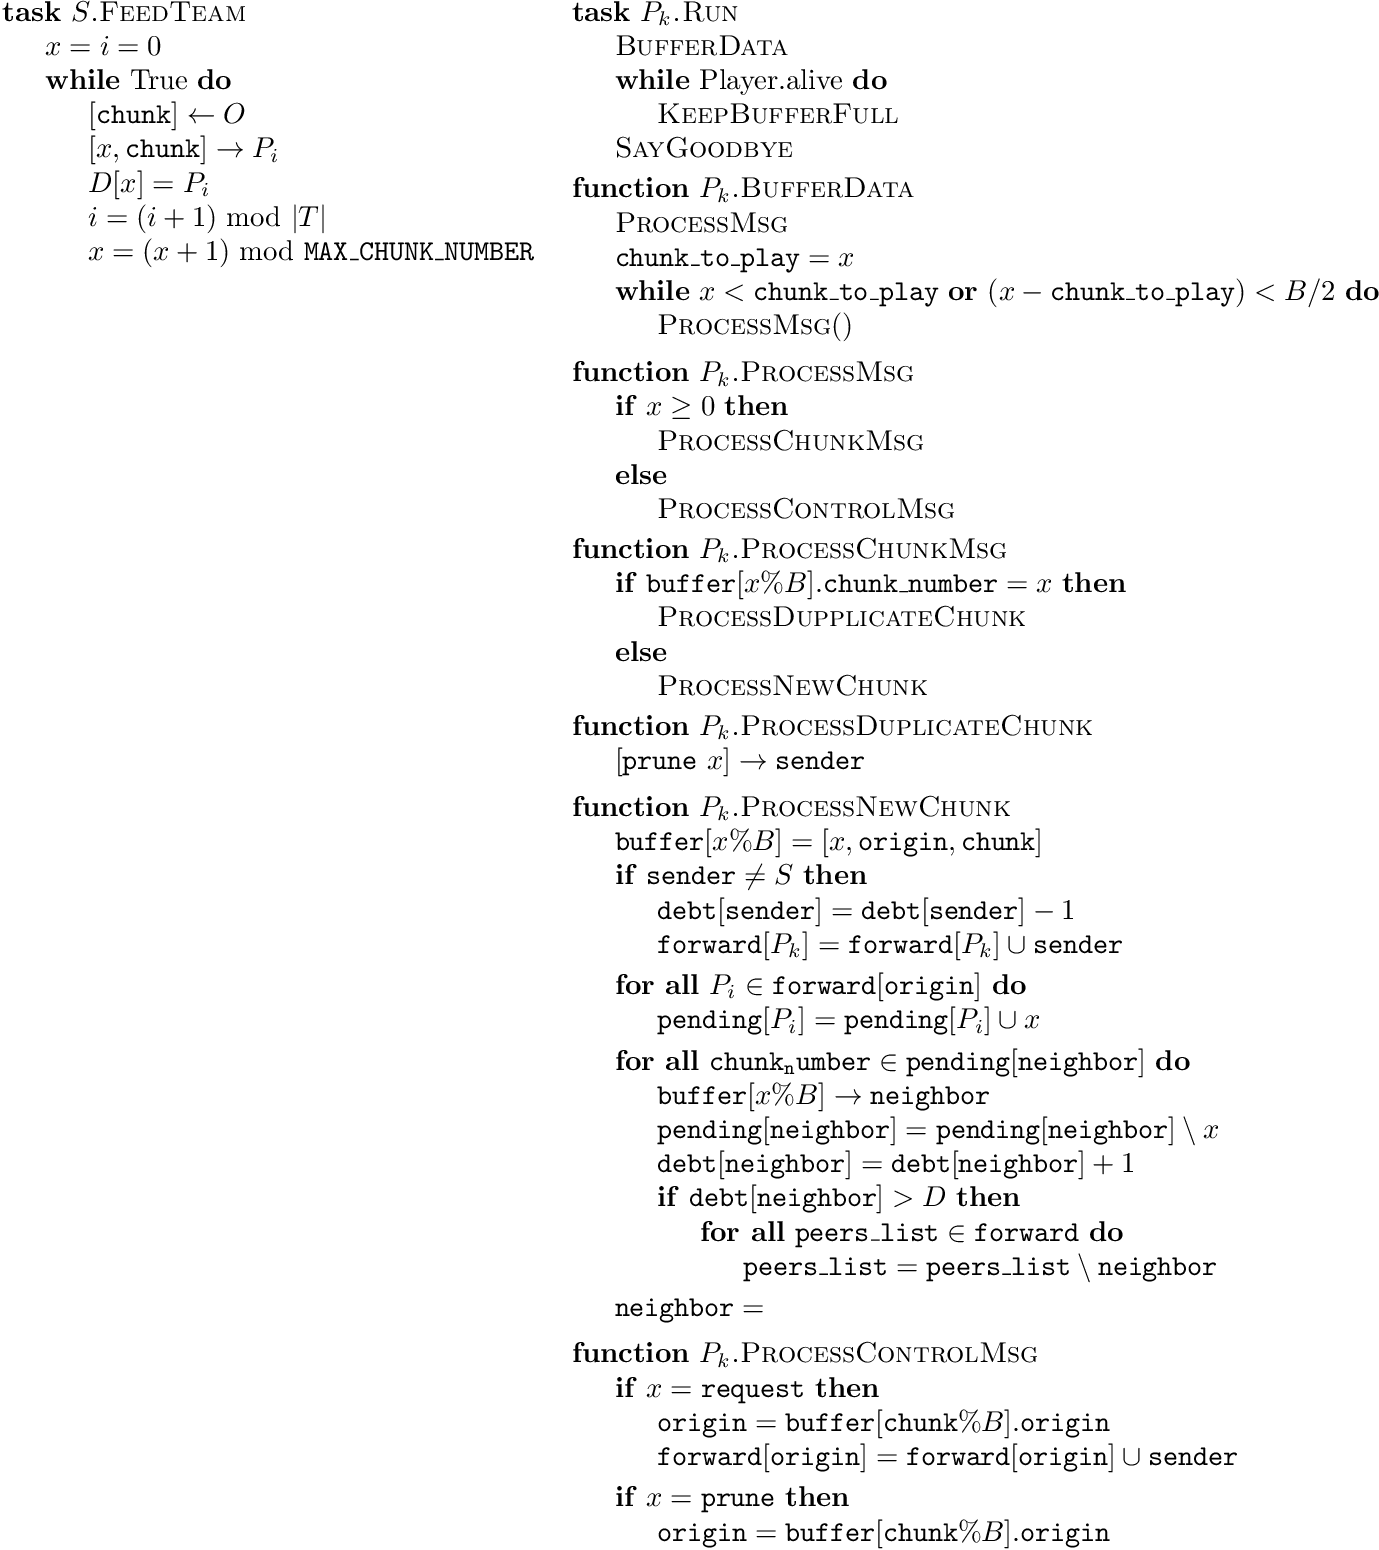
\includegraphics[width=0.75\textwidth]{chunk_generation_and_flooding}
  \fig{500}{5cm}{DBS_splitter_feed} \caption{Chunk
    generation at the splitter and their transmission to the
    team.\label{fig:chunk_generation}}
\end{figure*}
\end{comment}

We define a \gls{round} as the process of transmitting $N$ different
chunks from the splitter to a team of $N\leq N^*$ peers (therefore,
all the peers of the team are origin of a different chunk, in each
round). For a team of size $N$, the \gls{round-time} can be estimated
as
\begin{equation}
  t_r=Nt_c.
\end{equation}
Notice that $t_r$ is generally variable, and depends on
the current number of peers in the team ($N$). The
\gls{chunk-time} is defines as 
\begin{equation}
  \label{eq:chunk_time}
  t_c=\frac{C}{R},
\end{equation}
which depends on the chunk size $C$ and the average bit-rate of the
media stream $R$.

\begin{comment}
(in a team) as the time necessary to send two consecutive chunks from
  the splitter (of such team) to the same peer, using the
  round-robing. This time is variable and depends on $|T|$, $C$, and
  the average bit-rate of the media, $A$.
\end{comment}

\begin{comment}
The round-time is defined by:
\begin{equation}
  \cal{r} = \cal{c}N.
  \label{eq:round_time}
\end{equation}
For example, if we use only one team of $N=256$ peers, a chunk size
$C=1024$~bytes, and a video of $1$~Mb/s, the round time is
\begin{displaymath}
  \cal{r} = \frac{1024\frac{\text{bytes}}{\text{chunk}}\times
    8\frac{\text{bits}}{\text{byte}}}{10^6\frac{\text{bits}}{\text{second}}}\times
  256 \approx 2.1~\text{seconds}.
\end{displaymath}
\end{comment}
